\section{空间曲线}

\subsection{正则曲线,弧长参数,单位切向量,曲率,主法向量,次法向量,挠率,Frenet 公式}

对于 $\mathbb{R}^3$ 中的正则曲线 ($\boldsymbol{r}'(t)\neq0$) $C:\boldsymbol{r}=\boldsymbol{r}(t),a\leq t\leq b$,引进参数 $s$ 使得
\[
s=s(t)=\int_{a}^{t} \lvert \boldsymbol{r}'(t) \rvert  \, dt
\]
$s$ 被称为曲线 $C$ 的 (弧长参数. 一个显然的事实是,正则曲线 $C:\boldsymbol{r}=\boldsymbol{r}(t)$ 的参数 $t$ 为正则参数的特征是 $\lvert \boldsymbol{r}'(t) \rvert\equiv1$. 一般的计算中,$t$ 未必是弧长参数.

关于空间曲线的理论,最重要的是沿曲线 $\boldsymbol{r}=\boldsymbol{r}(t)$ 定义的 Frenet 标架 $\{ \boldsymbol{r};\boldsymbol{\alpha},\boldsymbol{\beta},\boldsymbol{\gamma} \}$ 和 Frenet 公式.

假定空间曲线 $C$ 的参数方程为 $\boldsymbol{r}=\boldsymbol{r}(s)$,其中 $s$ 是弧长参数,那么它的

单位切向量:
\[
\boldsymbol{\alpha}(s)=\boldsymbol{r}'(s)
\]
曲率:
\[
\kappa(s)=\lvert \boldsymbol{\alpha}'(s) \rvert =\lvert \boldsymbol{r}''(s) \rvert 
\]
曲率非零时,主法向量 (这样的定义是自然的):
\[
\boldsymbol{\beta}(s)=\frac{\boldsymbol{\alpha}'(s)}{\lvert \boldsymbol{\alpha}'(s) \rvert }=\frac{\boldsymbol{r}''(s)}{\lvert \boldsymbol{r}''(s) \rvert }
\]
次法向量:
\[
\boldsymbol{\gamma}(s)=\boldsymbol{\alpha}(s)\times \boldsymbol{\beta}(s)
\]
挠率\footnote{挠率一开始的定义就是使得 $\boldsymbol{\gamma}'(s)=-\tau(s)\boldsymbol{\beta}(s)$ 的 $s$ 函数,下面这个只是计算式.}
\[
\tau(s)=-\boldsymbol{\gamma}'(s)\cdot\boldsymbol{\beta}(s)
\]
曲线的 Frenet 公式是
\[
\begin{cases}
\boldsymbol{r}^{\prime}(s) &= \boldsymbol{\alpha}(s), \\
\boldsymbol{\alpha}^{\prime}(s) &= \kappa(s) \boldsymbol{\beta}(s), \\
\boldsymbol{\beta}^{\prime}(s) &= -\kappa(s) \boldsymbol{\alpha}(s) + \tau(s) \boldsymbol{\gamma}(s), \\
\boldsymbol{\gamma}^{\prime}(s) &= -\tau(s) \boldsymbol{\beta}(s),
\end{cases}
\]
上式都是关于弧长参数 $s=\int_{a}^{t} \lvert \boldsymbol{r}'(t) \rvert \, dt$ 的导数.

\subsubsection{Frenet 公式推导}

首先根据 $\boldsymbol{\alpha}(s)$ 定义知道 $\boldsymbol{r}'(s)=\boldsymbol{\alpha}(s)$. 其次根据 $\kappa(s),\boldsymbol{\beta}(s)$ 的定义知道
\[
\kappa(s)\boldsymbol{\beta}(s)=\boldsymbol{r}''(s)=\boldsymbol{\alpha}'(s)
\]
根据 $\tau(s)$ 最原本的定义可知
\[
\boldsymbol{\gamma}'(s)=-\tau(s)\boldsymbol{\beta}(s)
\]
接下来待定系数求解 $\boldsymbol{\beta}'(s)=a\boldsymbol{\alpha}(s)+b\boldsymbol{\beta}(s)+c\boldsymbol{\gamma}(s)$,分别与 $\boldsymbol{\alpha}(s),\boldsymbol{\beta}(s),\boldsymbol{\gamma}(s)$ 作内积得到
\[
\begin{aligned}
a & =\boldsymbol{\beta}'(s)\cdot\boldsymbol{\alpha}(s)\overset{ \boldsymbol{\alpha}(s)\bot\boldsymbol{\beta}(s) }{ = }-\boldsymbol{\beta}(s)\cdot\boldsymbol{\alpha}'(s)=-\kappa(s) \\
b & =\boldsymbol{\beta}'(s)\cdot\boldsymbol{\beta}(s)=0 \\
c & =\boldsymbol{\beta}'(s)\cdot\boldsymbol{\gamma}(s)\overset{ \boldsymbol{\beta}(s)\bot\boldsymbol{\gamma}(s) }{ = }-\boldsymbol{\beta}(s)\cdot\underbrace{ \boldsymbol{\gamma}'(s) }_{ =-\tau(s)\boldsymbol{\beta}(s) }=\tau(s)
\end{aligned}
\]
从而
\[
\boldsymbol{\beta}'(s)=-\kappa(s)\boldsymbol{\alpha}(s)+\tau(s)\boldsymbol{\gamma}(s)
\]
我们完成了 Frenet 公式的推导证明!

\subsection{转化为关于 \texorpdfstring{$t$}{t} 的方程}

在曲线的一般参数下,设曲线的参数方程是 $\boldsymbol{r}=\boldsymbol{r}(t)$ ,则它的单位切向量是
\[
\boldsymbol{\alpha}(t)=\frac{\boldsymbol{r}^{\prime}(t)}{\left|\boldsymbol{r}^{\prime}(t)\right|}
\]
假定曲线的弧长参数是 $s$ ,则 $s^{\prime}(t)=\left|\boldsymbol{r}^{\prime}(t)\right|$ ,所以
\[
\boldsymbol{r}^{\prime}(t)=\frac{\mathrm{d} \boldsymbol{r}(t)}{\mathrm{d} s} \frac{\mathrm{~d} s}{\mathrm{~d} t}=\boldsymbol{\alpha}(t) s^{\prime}(t)
\]
因此
\[
\begin{aligned}
r^{\prime \prime}(t) & =\frac{\mathrm{d} \boldsymbol{\alpha}(t)}{\mathrm{d} t} s^{\prime}(t)+\boldsymbol{\alpha}(t) s^{\prime \prime}(t) \\
& =\frac{\mathrm{d} \boldsymbol{\alpha}(t)}{\mathrm{d} s}\left(s^{\prime}(t)\right)^2+\boldsymbol{\alpha}(t) s^{\prime \prime}(t) \\
& =\kappa(t) \boldsymbol{\beta}(t)\left(s^{\prime}(t)\right)^2+\boldsymbol{\alpha}(t) s^{\prime \prime}(t),
\end{aligned}
\]
故
\[
\boldsymbol{r}^{\prime}(t) \times \boldsymbol{r}^{\prime \prime}(t)=\kappa(t)\left(s^{\prime}(t)\right)^3 \boldsymbol{\alpha}(t) \times \boldsymbol{\beta}(t)=\kappa(t)\left(s^{\prime}(t)\right)^3 \boldsymbol{\gamma}(t)
\]
由此得到曲线的曲率是
\[
\kappa(t)=\frac{\left|\boldsymbol{r}^{\prime}(t) \times \boldsymbol{r}^{\prime \prime}(t)\right|}{\left(s^{\prime}(t)\right)^3}=\frac{\left|\boldsymbol{r}^{\prime}(t) \times \boldsymbol{r}^{\prime \prime}(t)\right|}{\left|\boldsymbol{r}^{\prime}(t)\right|^3}
\]
次法向量是
\[
\gamma(t)=\frac{\boldsymbol{r}^{\prime}(t) \times \boldsymbol{r}^{\prime \prime}(t)}{\left|\boldsymbol{r}^{\prime}(t) \times \boldsymbol{r}^{\prime \prime}(t)\right|}
\]
这样,曲线的主法向量是
\[
\boldsymbol{\beta}(t)=\boldsymbol{\gamma}(t) \times \boldsymbol{\alpha}(t)
\]
再利用 Frenet 公式得到
\[
\begin{aligned}
\tau(t) & =-\left(\boldsymbol{\gamma}^{\prime}(t) \frac{\mathrm{d} t}{\mathrm{~d} s}\right) \cdot \boldsymbol{\beta}(t)=-\frac{1}{\left|\boldsymbol{r}^{\prime}(t)\right|} \boldsymbol{\gamma}^{\prime}(t) \cdot \boldsymbol{\beta}(t) \\
& =\frac{\left(\boldsymbol{r}^{\prime}(t), \boldsymbol{r}^{\prime \prime}(t), \boldsymbol{r}^{\prime \prime \prime}(t)\right)}{\left|\boldsymbol{r}^{\prime}(t) \times \boldsymbol{r}^{\prime \prime}(t)\right|^2}
\end{aligned}
\]
此时,单位切向量,主法向量和次法向量的导数是
\[
\begin{aligned}
& \boldsymbol{\alpha}^{\prime}(t)=\frac{\mathrm{d} \boldsymbol{\alpha}}{\mathrm{~d} s} \cdot s^{\prime}(t)=\kappa(t) s^{\prime}(t) \boldsymbol{\beta}(t), \\
& \boldsymbol{\beta}^{\prime}(t)=\frac{\mathrm{d} \boldsymbol{\beta}}{\mathrm{~d} s} \cdot s^{\prime}(t)=-\kappa(t) s^{\prime}(t) \boldsymbol{\alpha}(t)+\tau(t) s^{\prime}(t) \boldsymbol{\gamma}(t), \\
& \boldsymbol{\gamma}^{\prime}(t)=\frac{\mathrm{d} \boldsymbol{\gamma}}{\mathrm{~d} s} \cdot s^{\prime}(t)=-\tau(t) s^{\prime}(t) \boldsymbol{\beta}(t) .
\end{aligned}
\]
\begin{theorem}[空间曲线基本定理]
给定两个连续可微函数 $\kappa(s),\tau(s)$ 其中 $\kappa(s)>0$,则在三维欧式空间中存在一条空间曲线,以 $s$ 为弧长参数,以 $\kappa(s)$ 为曲率,以 $\tau(s)$ 为挠率,并且这样的曲线的形状是完全确定的.
\end{theorem}
\begin{remark}
在给定 $\kappa(s),\tau (s)$ 的情况下,Frenet 公式构成了向量 $\boldsymbol{r},\boldsymbol{\alpha},\boldsymbol{\beta},\boldsymbol{\gamma}$ 的微分方程组,可以求解.
\end{remark}
\subsection{切触阶}

两条相交曲线在交点附近的接近程度是用所谓的\textbf{切触阶}来刻画的.
\begin{figure}[H]
\centering
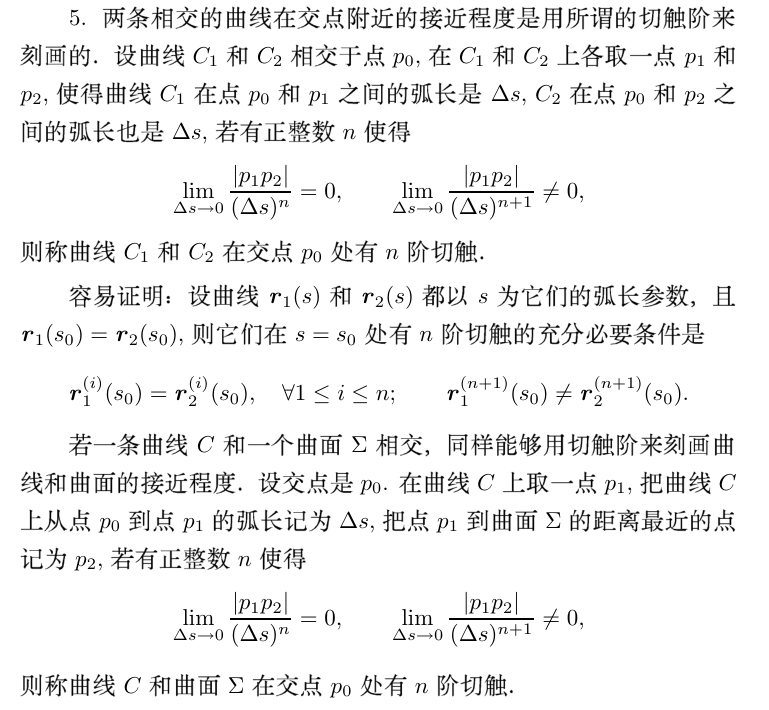
\includegraphics[width=\textwidth]{3-空间曲线(不严谨)-2025040423.png}
% \caption{}
\label{}
\end{figure}

\subsection{平面曲线}

平面曲线可以看作空间曲线的特例,即 $\tau(s)\equiv0$ 的空间曲线. 空间曲线求曲率 $\kappa(s)=\lvert \boldsymbol{r}''(s) \rvert$ 的公式照用. 特别的是,平面本身\textbf{有定向},将其单位切向量正向 (逆时针) 旋转 $90\degree$ 便得到法向量 (唯一确定). 于是
\[
\boldsymbol{\alpha}(s)=(x'(s),y'(s))
\]
正向旋转 $90\degree$ 得到\footnote{不一定是主法向量}
\[
\boldsymbol{\beta}(s)=(-y'(s),x'(s))
\]
相对曲率
\[
\kappa_{r}(s)=\boldsymbol{\alpha}'(s)\cdot\boldsymbol{\beta}(s)=x'(s)y''(s)-y'(s)x''(s)
\]
相对曲率 $\kappa_{r}$ 与曲率 $\kappa$ 的关系是 $\kappa_{r}=\pm\kappa$. 正号表示曲线朝着 $\boldsymbol{\beta}(s)$ 的方向弯曲,负号表示曲线的主法向量为 $-\boldsymbol{\beta}(s)$.

\subsection{例题}

\subsubsection{已知参数方程求曲线方程}

\subsubsection{已知一般方程求参数方程}

\subsubsection{已知曲线方程求曲线曲率、挠率、Frenet 标架}

已知参数方程,直接套公式爆算:
\begin{figure}[H]
\centering
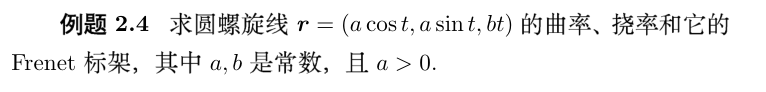
\includegraphics[width=\textwidth]{3-空间曲线(不严谨)-2025040322.png}
% \caption{}
\label{}
\end{figure}
已知一般方程:
\begin{figure}[H]
\centering
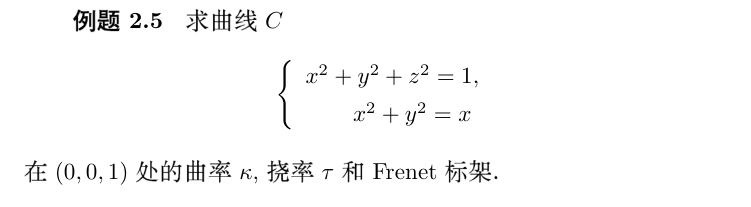
\includegraphics[width=\textwidth]{空间曲线(不严谨)-2025040322.png}
% \caption{}
\label{}
\end{figure}
直接通过对方程求导,求解出 $\boldsymbol{r}'(0),\boldsymbol{r}''(0),\boldsymbol{r}'''(0)$.
\begin{figure}[H]
\centering
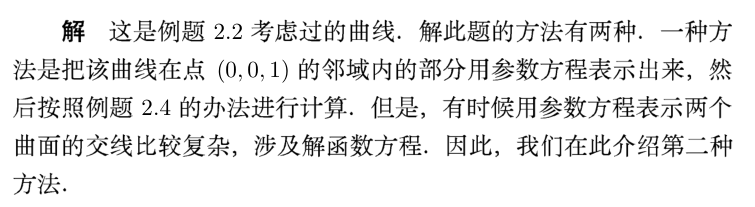
\includegraphics[width=\textwidth]{2-空间曲线(不严谨)-2025040322.png}
% \caption{}
\label{}
\end{figure}

\subsubsection{求解新曲线的曲率、挠率、Frenet 标架}

\begin{figure}[H]
\centering
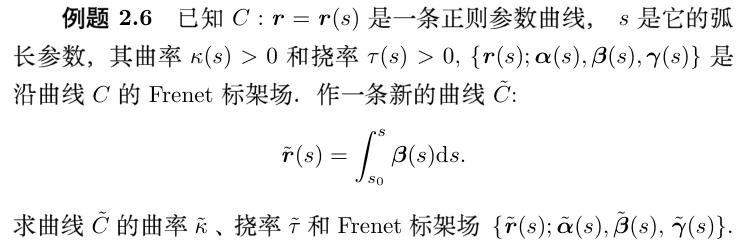
\includegraphics[width=\textwidth]{4-空间曲线(不严谨)-2025040322.png}
% \caption{}
\label{}
\end{figure}

\begin{figure}[H]
\centering
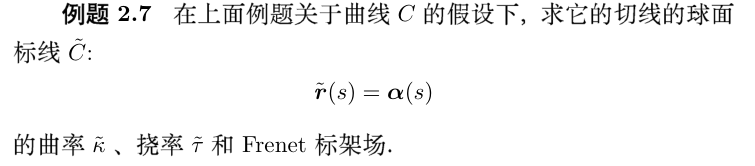
\includegraphics[width=\textwidth]{5-空间曲线(不严谨)-2025040322.png}
% \caption{}
\label{}
\end{figure}

\subsubsection{特定曲线满足曲率挠率关系式}

\begin{figure}[H]
\centering
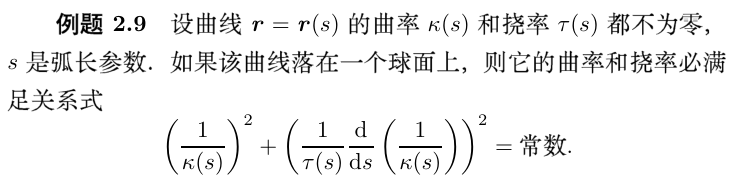
\includegraphics[width=\textwidth]{6-空间曲线(不严谨)-2025040322.png}
% \caption{}
\label{}
\end{figure}

\begin{figure}[H]
\centering
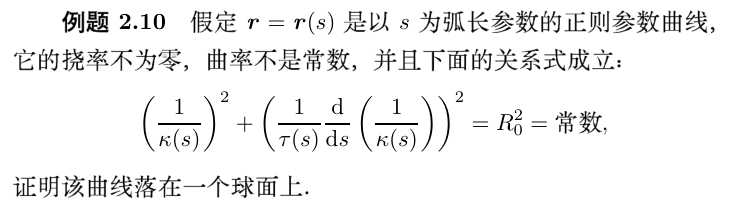
\includegraphics[width=\textwidth]{7-空间曲线(不严谨)-2025040322.png}
% \caption{}
\label{}
\end{figure}

\subsubsection{已知曲率挠率,求解曲线参数方程}

\begin{figure}[H]
\centering
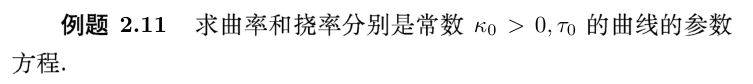
\includegraphics[width=\textwidth]{8-空间曲线(不严谨)-2025040322.png}
% \caption{}
\label{}
\end{figure}

根据曲线论基本定理具有这样常数曲率 $\kappa_0>0$ 和挠率 $\tau_0$ 的曲线必定是圆螺旋线
\[
\boldsymbol{r}=(a\cos t,a\sin t,bt)\qquad a>0,b\text{ 是常数}
\]
\begin{remark}
本题也可以根据 Frenet 标架直接求解微分方程组.
\end{remark}
\subsubsection{求密切圆}

\begin{figure}[H]
\centering
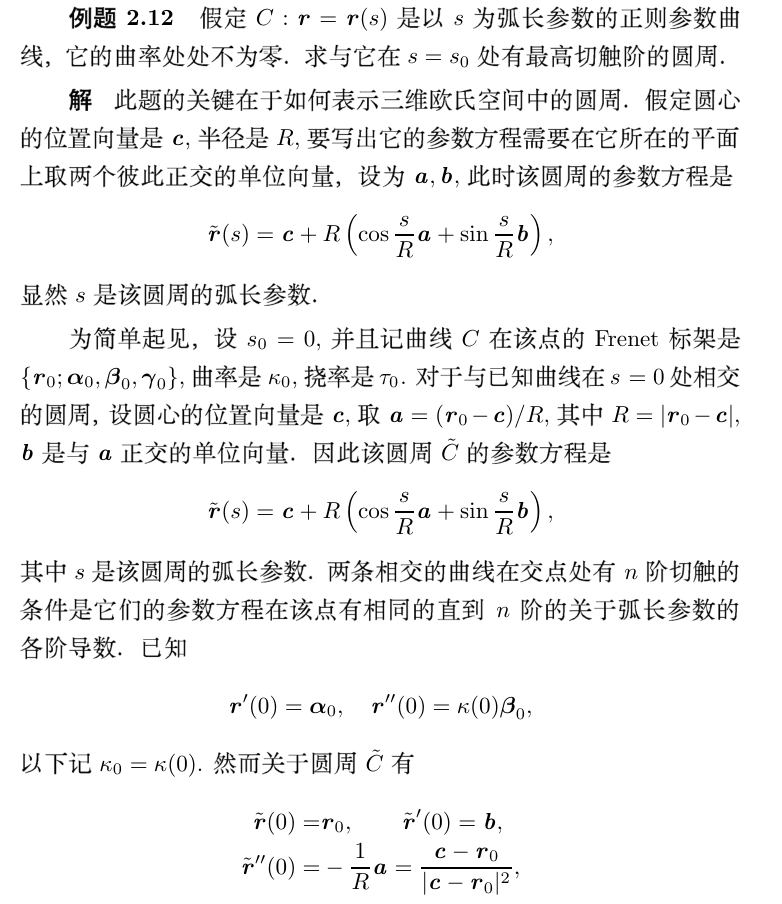
\includegraphics[width=\textwidth]{9-空间曲线(不严谨)-2025040322.png}
% \caption{}
\label{}
\end{figure}

\begin{figure}[H]
\centering
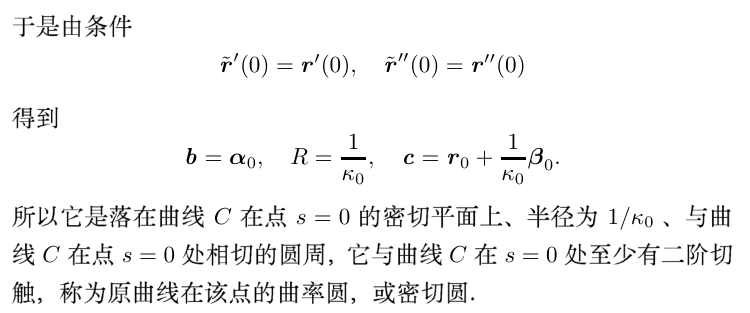
\includegraphics[width=\textwidth]{10-空间曲线(不严谨)-2025040322.png}
% \caption{}
\label{}
\end{figure}

\subsubsection{求密切球}

\begin{figure}[H]
\centering
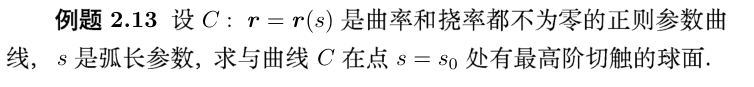
\includegraphics[width=\textwidth]{11-空间曲线(不严谨)-2025040322.png}
% \caption{}
\label{}
\end{figure}

\subsubsection{求渐伸线和渐缩线参数方程}

\begin{figure}[H]
\centering
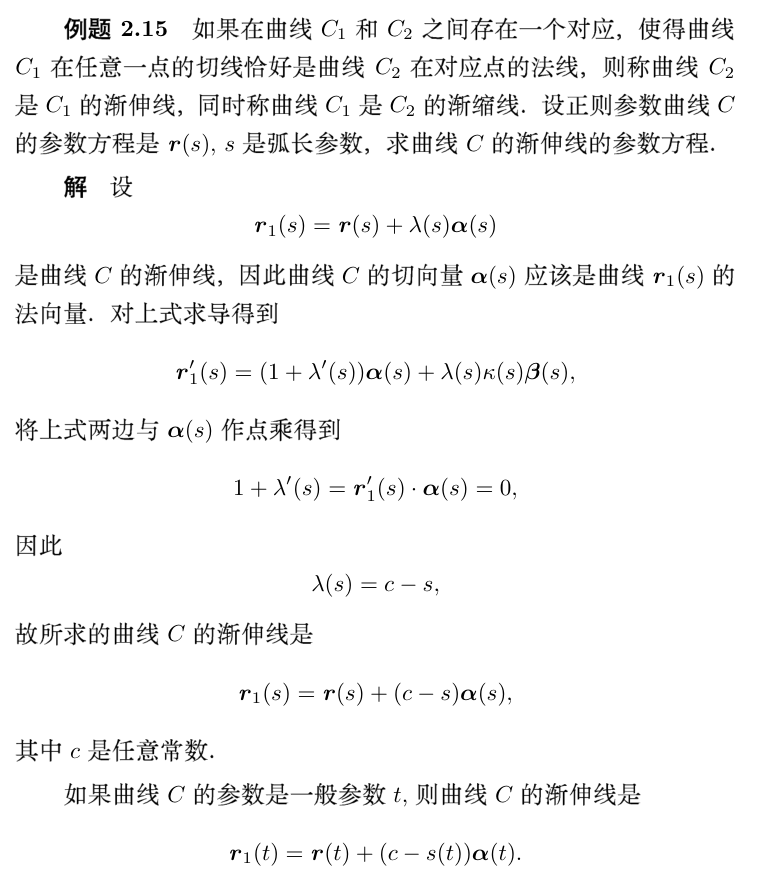
\includegraphics[width=\textwidth]{12-空间曲线(不严谨)-2025040322.png}
% \caption{}
\label{}
\end{figure} \begin{figure}[H]
\centering
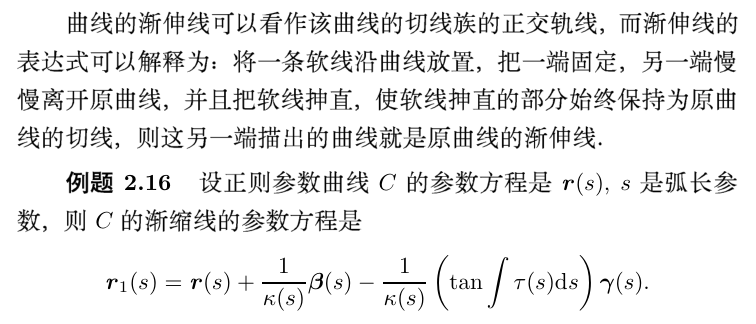
\includegraphics[width=\textwidth]{13-空间曲线(不严谨)-2025040322.png}
% \caption{}
\label{}
\end{figure}
\begin{figure}[H]
\centering
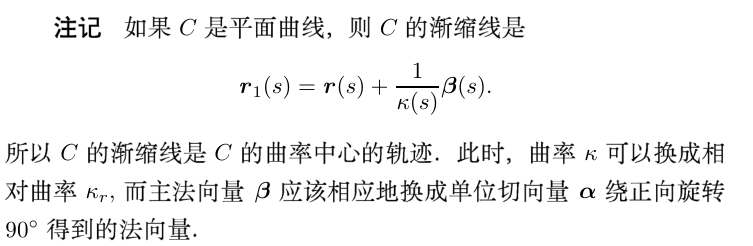
\includegraphics[width=\textwidth]{14-空间曲线(不严谨)-2025040322.png}
% \caption{}
\label{}
\end{figure}
